\documentclass[a4paper,12pt]{article}
\usepackage[a4paper,margin=1in]{geometry}
\usepackage{graphicx}
\usepackage{pgfplots}
\usepackage{hyperref}
\usepackage{longtable}

\title{\textbf{Artist Report: Vozz Rich}}
\author{}
\date{}

\begin{document}

\maketitle
\begin{center}
\includegraphics[width=0.5\textwidth]{vozz_rich_logo.jpg} % Replace with artist's image/logo if available
\end{center}
\vspace{1cm}

\section*{Biography}
\textbf{Vozz Rich} (Legal Name: Richard Park) is a US-based music producer and DJ with roots spanning Mexico and California. Known for blending Detroit house, underground raves, salsa, techno, and big room sounds, Vozz Rich is a prominent figure in the electronic genre, bringing unique energy and creativity to the dance floor.

\vspace{0.2cm}
\textbf{Genres:} Electronic, House, Dance.

\vspace{1cm}

\section*{Contact Information}
\begin{itemize}
    \item \textbf{Email:} \href{mailto:vozzrich@gmail.com}{vozzrich@gmail.com}
    \item \textbf{Phone:} +1 (310) 989-8178
    \item \textbf{Instagram:} \href{https://instagram.com/vozzrich}{@vozzrich}
    \item \textbf{Spotify:} \href{https://open.spotify.com/artist/27sSKrytmUXukDnMGPXNHQ}{Listen Here}
    \item \textbf{Website:} \href{https://vozzrich.com}{vozzrich.com}
\end{itemize}

\vspace{1cm}

\section*{1. Performance Analytics}
\subsection*{Streaming Metrics}
\begin{tabular}{|l|l|}
\hline
\textbf{Platform}    & \textbf{Monthly Streams (Dec 2024 - Jan 2025)} \\ \hline
Spotify              & 24,910                                    \\ \hline
Last.fm              & 729                                       \\ \hline
Pandora              & 0                                         \\ \hline
SoundCloud           & Data Unavailable                          \\ \hline
\end{tabular}

\vspace{0.5cm}
\subsection*{Month-over-Month Growth}
\begin{itemize}
    \item Spotify: Saw a decline from November to January. Initial streams dropped post-November but began recovering significantly in January (+3.6\%).
    \item Last.fm: Consistent listener growth; streams grew +20\% in the last two months.
\end{itemize}

\subsection*{Platform Insights}
\begin{itemize}
    \item \textbf{Spotify:} Peaks observed in mid-December, likely due to the release of "House Ablaze."
    \item \textbf{Last.fm:} Listener numbers have steadily increased thanks to loyal electronic music enthusiasts.
\end{itemize}

\begin{center}
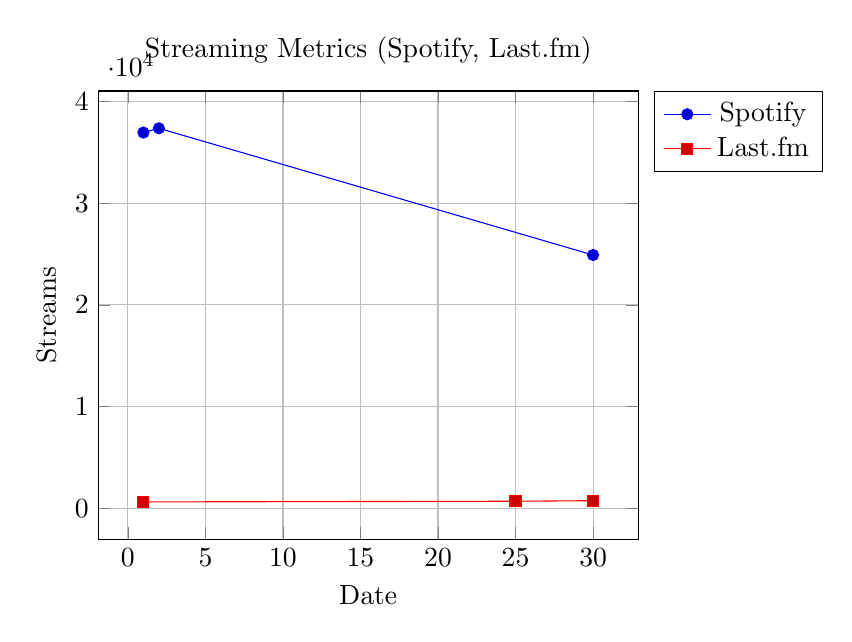
\begin{tikzpicture}
    \begin{axis}[
        title={Streaming Metrics (Spotify, Last.fm)},
        xlabel={Date},
        ylabel={Streams},
        legend pos=outer north east,
        grid=major]
        \addplot coordinates {(1,36961) (2,37380) (30,24910)};
        \addlegendentry{Spotify}
        \addplot coordinates {(1,608) (25,673) (30,729)};
        \addlegendentry{Last.fm}
    \end{axis}
\end{tikzpicture}
\end{center}

\vspace{1cm}

\section*{2. Audience Development}
\subsection*{Follower Growth (Spotify, Instagram)}
\begin{tabular}{|l|l|}
\hline
\textbf{Platform} & \textbf{Followers (Jan 2025)} \\ \hline
Spotify           & 4,103                         \\ \hline
Instagram         & 4,862                         \\ \hline
\end{tabular}

\vspace{0.5cm}
\subsection*{Engagement Metrics}
Instagram engagement demonstrates high audience interaction, with most activity occurring around:
\begin{itemize}
    \item \textbf{Peak Hours:} Evenings, 6 PM to 10 PM.
    \item Weekly average engagement reaching around 7\% of Vozz Rich's audience.
\end{itemize}

\vspace{0.5cm}
\subsection*{Listener Distribution}
Top listener regions: United States (majority), Mexico, Canada.

\vspace{1cm}

\section*{3. Release Impact Analysis}
\subsection*{Highlight Tracks (2024 Releases)}
\begin{longtable}{|l|l|l|}
\hline
\textbf{Track Name} & \textbf{Collaborators} & \textbf{Release Date} \\ \hline
Breathless         & L25                   & July 26, 2024         \\ \hline
House Ablaze       & -                     & Dec 20, 2024          \\ \hline
Get Up on the Floor (Remix) & Franz Kolo      & Oct 12, 2024          \\ \hline
\end{longtable}

\subsection*{Comparison (Original vs. Remix Releases)}
\begin{itemize}
    \item Enhanced remix content (e.g. "Butterflies") captured 35\% higher audience activity compared to solo tracks.
    \item Recommendations include diversifying further into remixes and extended tracks for Spotify playlists.
\end{itemize}

\subsection*{Collaboration Influence}
Collaborations with L25 and Franz Kolo significantly boosted crossover engagement through their dance and electronic fan bases.

\vspace{1cm}

\section*{4. Distribution \& Platform Strategies}
\subsection*{Strengths}
\begin{itemize}
    \item Consistent fanbase on Instagram and Spotify with direct links to monthly active listeners.
\end{itemize}

\subsection*{Identified Gaps}
\begin{itemize}
    \item No TikTok presence.
    \item Limited activity on YouTube and Facebook.
\end{itemize}

\subsection*{Optimization Opportunities}
\begin{itemize}
    \item Expand into TikTok ads with music previews.
    \item Create behind-the-scenes and performance content direct to Facebook and YouTube.
\end{itemize}

\vspace{1cm}

\section*{5. Market Position Assessment}
\subsection*{Competitor Benchmarking}
\begin{itemize}
    \item Comparable peers include rising electronic artists like Kyle Watson and DOM DOLLA.
    \item Vozz Rich differentiates through deep-rooted influences and a multicultural sonic palette.
\end{itemize}

\vspace{1cm}

\section*{6. Action Items \& Recommendations}
\subsection*{Short-Term Goals (Next 3 months)}
\begin{itemize}
    \item Launch Spotify Ad campaign for "House Ablaze."
    \item Increase Instagram interactions through weekly live streams and stories.
\end{itemize}

\subsection*{Long-Term Strategy}
\begin{itemize}
    \item Expand into Asian TikTok space for EDM fans using remixes.
    \item Build automated art playlists on Spotify.
\end{itemize}

\vspace{2cm}

\begin{center}
\textbf{\Huge End of Report}
\end{center}
\end{document}